%!TEX root = ../main.tex
\chapter{Introduzione}\label{chp:introduction}

Ad oggi l'avanzamento della genomica — branca della biologia molecolare che si occupa di studiare il genoma degli esseri viventi — si è rivelato notevolmente significativo al fine di approfondire e comprendere malattie legate alle mutazioni del genoma degli individui. Si stima che solamente una percentuale tra l'1\% e il 2\% del DNA contiene i \textsl{geni}, ovvero particolari regioni che contengono tutte le informazioni necessarie per la sintesi degli aminoacidi che poi comporranno le proteine\,\cite{sahu2011identification}. Ciò nonostante, la quasi totalità dei disturbi genomici è dovuta alle mutazioni nelle regioni non codificanti\,\cite{zhang2015non} — dette \textsl{varianti non codificianti}. Le mutazioni in queste zone del genoma, che apparentemente svolgono funzioni marginali, sono responsabili dello sviluppo di disturbi importanti, come le \textsl{malattie mendeliane}\footnote{Le malattie mendeliane, causate dalla mutazione di un singolo gene, includono la fibrosi cistica e il morbo di Huntington.}\,\cite{french2020role, chial2008mendelian}, l'epilessia\,\cite{pagni2022non}, malattie cardiovascolari\,\cite{kapoor2014enhancer, zhang2015non} e soprattuto tumori — tra cui il cancro del colon-retto e tumore al seno\,\cite{khurana2016role, tian2019systematic, bojesen2013multiple, michailidou2017association}.

Risulta quindi vitale continuare a studiare gli effetti che le varianti non codificanti in sequenze genomiche hanno sugli individui. Proprio a questo proposito, con l'avvento dell'intelligenza artificiale, in particolare del \textsl{deep learning}, si continuano a trovare e perfezionare soluzioni che permettano di delineare sempre con più precisione il ruolo che hanno le mutazioni nelle regioni non codificanti del DNA.\@ Grazie a queste nuove tecnologie, la \textsl{genomica funzionale} — area della genomica che si interessa a descrivere le relazioni che ci sono tra i componenti di un sistema biologico, come geni e proteine\,\cite{caudai2021ai} — ha avuto un forte impulso nell'approfondire le varianti non codificanti ma rimangono ancora significative lacune nella comprensione riguardante la relazione tra mutazioni genetiche ed espressione genica. L'utilizzo di tecniche di deep learning quindi cruciale per continuare la ricerca; a questo proposito, nel presente elaborato accademico verranno descritti e paragonati tre \textsl{tool} che utilizzano le \textsl{reti neurali convoluzionali} per predire l'effetto delle varianti non codificanti su sequenze genomiche: DeepSEA\,\cite{zhou2015predicting}, Basset\,\cite{kelley2016basset} e DeepSATA\,\cite{ma2023deepsata}.



\section{Background}

La cellula è l'unità fondamentale della vita. La cellula è una piccola miscela acquosa con componenti chimici, racchiusi in una mambrana, e possiede l'eccezionale capacità di replicarsi. Il primo elemento che permette di distinguere le cellule è la presenza di un nucleo. Vengono definite \textsl{procarioti} le cellule senza nucleo — che sono le più diffuse e compongono organismi unicellulari come i batteri e gli archei — mentre sono chiamate \textsl{eucarioti} le cellule che contengono un nucleo — le quali sono in genere più grandi e più complesse e costituiscono forme di vita multicellulari come animali piante e funghi\,\cite{alberts2015essential}.

All'interno della cellula eucariote sono presenti diversi \textsl{organuli}, i quali svolgono una particolare funzione ciascuno. I \textsl{mitocondri} sono gli organuli più diffusi all'interno del \textsl{citoplasma}. Il loro compito è quello di generare energia chimica per la cellula: attraverso il processo di ossidazione, trasformano; questo processo è chiamato respirazione cellulare.

Ciò nonostante, l'organulo più importante è il nucloe.
\todo{Plurifunctional nucleous\,\cite{pederson1998plurifunctional}}

\todo{il DNA si trova nel nucleo in forma compatta, i cromosomi.}


Il DNA è una molecola che si trova all'interno del nucleo di ciascuna cellula ed è composta, in una struttura a doppia elica, da \textsl{nucleotidi}. Osservando l'illustrazione\,\ref{fig:dna}, i nucleotidi sono composti a loro volta da tre elementi fondamentali: una \textsl{base azotata}, uno \textsl{zucchero} e un \textsl{gruppo fosfato}. Le basi azotate sono quattro — Adenina (A), Citosina (C), Guanina (G) e Timina (T) — e si legano tra loro secondo un preciso criterio: l'Adenina si lega solamente con la Timina (formando il legame \textit{AT}) mentre la Citosina si unisce solo con la Guanina (creando la coppia \textit{CG})\,\cite{fonseca2000hydrogen, sahu2011identification}.




\todo{parla dei geni, delle parti del gene in modo da spiegare bene le varianti non codificanti. se vuoi parla anche della funzione del dna del creare proteine descrivendo in breve il DNA}

\begin{figure}[h]
    \centering
    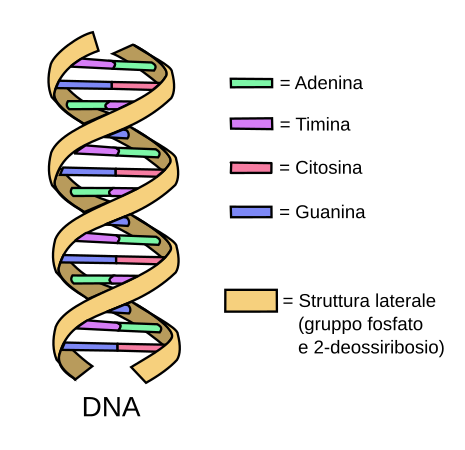
\includegraphics[width=.5\textwidth]{assets/DNA.png}
    \caption{Rappresentazione schematica del DNA\,\cite{forluvoft2012}.}
    \label{fig:dna}
\end{figure}


\todo{DNA replication\,\cite{bell2002dna}}

\section{Cenni storici}
\todo{
    C'è sto bell'articolo che racconta per bene la situa\cite{crick1954complementary, watson1953molecular, li2021cell}. Qua ci puoi buttare dentro anche la questione meme del junk DNA così pushi per bene le citazioni goliardiche.
}
\todo{ Sto libro parla anche della scopetrta delle cellule\cite{alberts2015essential}}


\section{Stato dell'arte}

\todo{parla dei tool e quanti ne sono uscit per letsgoscare le cose. Parla delle diversi vantaggi che AI ha portato nel letsgosky. Butta dentro deepvirfinder a anche alphafold perche fa figo\cite{ren2020identifying}}


% https://books.google.it/books?hl=it&lr=&id=Cg4WAgAAQBAJ&oi=fnd&pg=PP1&dq=Introduction+to+cell+biology&ots=yg4LdM46O3&sig=FkW8Ei_rOFccb96Sw3A28QsHuFo&redir_esc=y#v=onepage&q=Introduction%20to%20cell%20biology&f=false